% Created 2026-05-27 Wed 03:11
\documentclass{article}
\usepackage[utf8]{inputenc}
\usepackage[T1]{fontenc}
\usepackage{graphicx}
\usepackage{longtable}
\usepackage{wrapfig}
\usepackage{rotating}
\usepackage[normalem]{ulem}
\usepackage{amsmath}
\usepackage{amssymb}
\usepackage{capt-of}
\usepackage{hyperref}

\usepackage{fancyhdr}
\usepackage[top=25mm, left=25mm, right=25mm]{geometry}
\usepackage{longtable}
\fancyhead[R]{}
\setlength\headheight{43.0pt}
\usepackage{tabularx}
\usepackage{longtable}
\usepackage[backend=biber, style=ieee]{biblatex}
\addbibresource{/home/mateoijt-epn/RepoTrabajosGrupales/EPN-Lectures/iccd332ArqComp-2024-B/bibliography/bibliography.bib}
\author{Alex Flores, Micaela Sagñay, Molina Jhanavi, Jami Mateo}
\date{26/05/2026}
\title{Taller - Conceptos Básicos de Hardware y Ensamblaje de Computadores\\\medskip
\large ICCD332 Arquitectura de Computadores }
\hypersetup{
 pdfauthor={Alex Flores, Micaela Sagñay, Molina Jhanavi, Jami Mateo},
 pdftitle={Taller - Conceptos Básicos de Hardware y Ensamblaje de Computadores},
 pdfkeywords={},
 pdfsubject={},
 pdfcreator={Emacs 29.3 (Org mode 9.6.15)}, 
 pdflang={Spanish}}
\begin{document}

\maketitle
\fancyhead[C]{\includegraphics[scale=0.05]{../images/logoEPN.jpg}\\
ESCUELA POLITECNICA NACIONAL\\FACULTAD DE INGENIERIA DE SISTEMAS\\
ARQUITECTURA DE COMPUTADORES}
\thispagestyle{fancy}


\section{Instrucciones generales}
\label{sec:org0b25abf}

Este taller se realiza en \textbf{grupos}. Cada integrante debe completar
individualmente el curso Cisco Networking Academy:
\textbf{Conceptos Básicos de Hardware de Computadora} y obtener su
certificado de completitud. 

\textbf{Entregables del grupo:}
\begin{itemize}
\item Resolución de éste archivo fuente \texttt{.org}
\item El PDF exportado desde Emacs \texttt{M-x org-latex-export-to-pdf}
\item Los certificados individuales de cada integrante (PDF o imagen)
\end{itemize}


\textbf{Entregable Individual(Tarea):}
\begin{itemize}
\item Resolver el cuestionario individual en el aula virtual
\end{itemize}
\subsection{Recursos}
\label{sec:org2b2d58e}
Cree su usuario en la plataforma de \emph{Cisco Networking Academy}. Use el
siguiente enlace:

\href{https://www.netacad.com/es/courses/computer-hardware-basics?courseLang=en-US}{Cisco Computer Hardware Basics}

Puede configurar según el idioma de su preferencia. El texto está
disponible en Español. Los vídeos disponen de subtítulos en varios
idiomas.

\section{Parte A. Integrantes y certificados}
\label{sec:org6333d4b}
Para insertar la captura del certificado utilice YASnippet: Escriba
\texttt{fig\_} seguido de \texttt{C-TAB}. Esto produce \texttt{\#+caption}, \texttt{\#+attr\_latex} y
\texttt{\#+label} que permiten colocar un encabezado a la imagen, controlar el
escalado de la misma y una referencia. Finalmente inserte el enlace al
archivo usando \texttt{C-c C-l} o usando
\texttt{[[./carpeta-certificados/cert-int1.pdf]]}

\subsection{Integrante 1}
\label{sec:org8edc857}
\begin{itemize}
\item \textbf{Nombre completo:} Jhanavi Abigail Molina Gómez
\item \textbf{Correo:} jhanavi.molina@epn.edu.ec
\item \textbf{Certificado adjunto:}    
\begin{figure}[htbp]
\centering
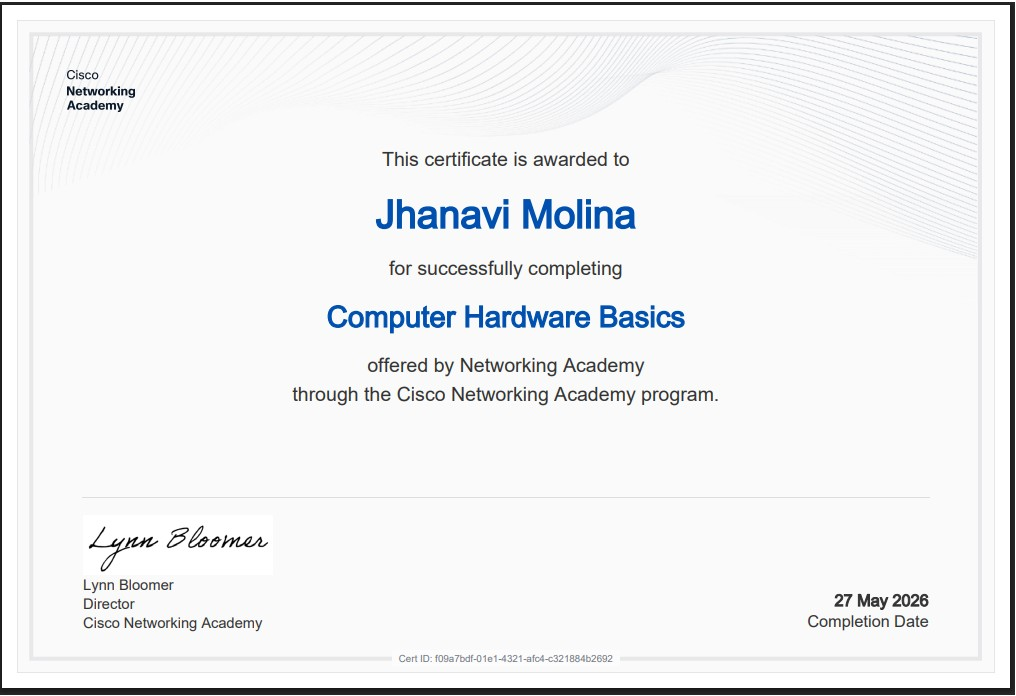
\includegraphics[width=.9\linewidth]{Certificado_Cisco.jpg}
\caption{\label{fig:org0ef6cb9}Certificado Molina Jhanavi}
\end{figure}
\end{itemize}


\subsection{Integrante 2}
\label{sec:org7a77688}
\begin{itemize}
\item \textbf{Nombre completo:} Alex Sebastian Flores Torres
\item \textbf{Correo:} alex.flores01@epn.edu.ec
\item \textbf{Certificado adjunto:}
\begin{figure}[htbp]
\centering
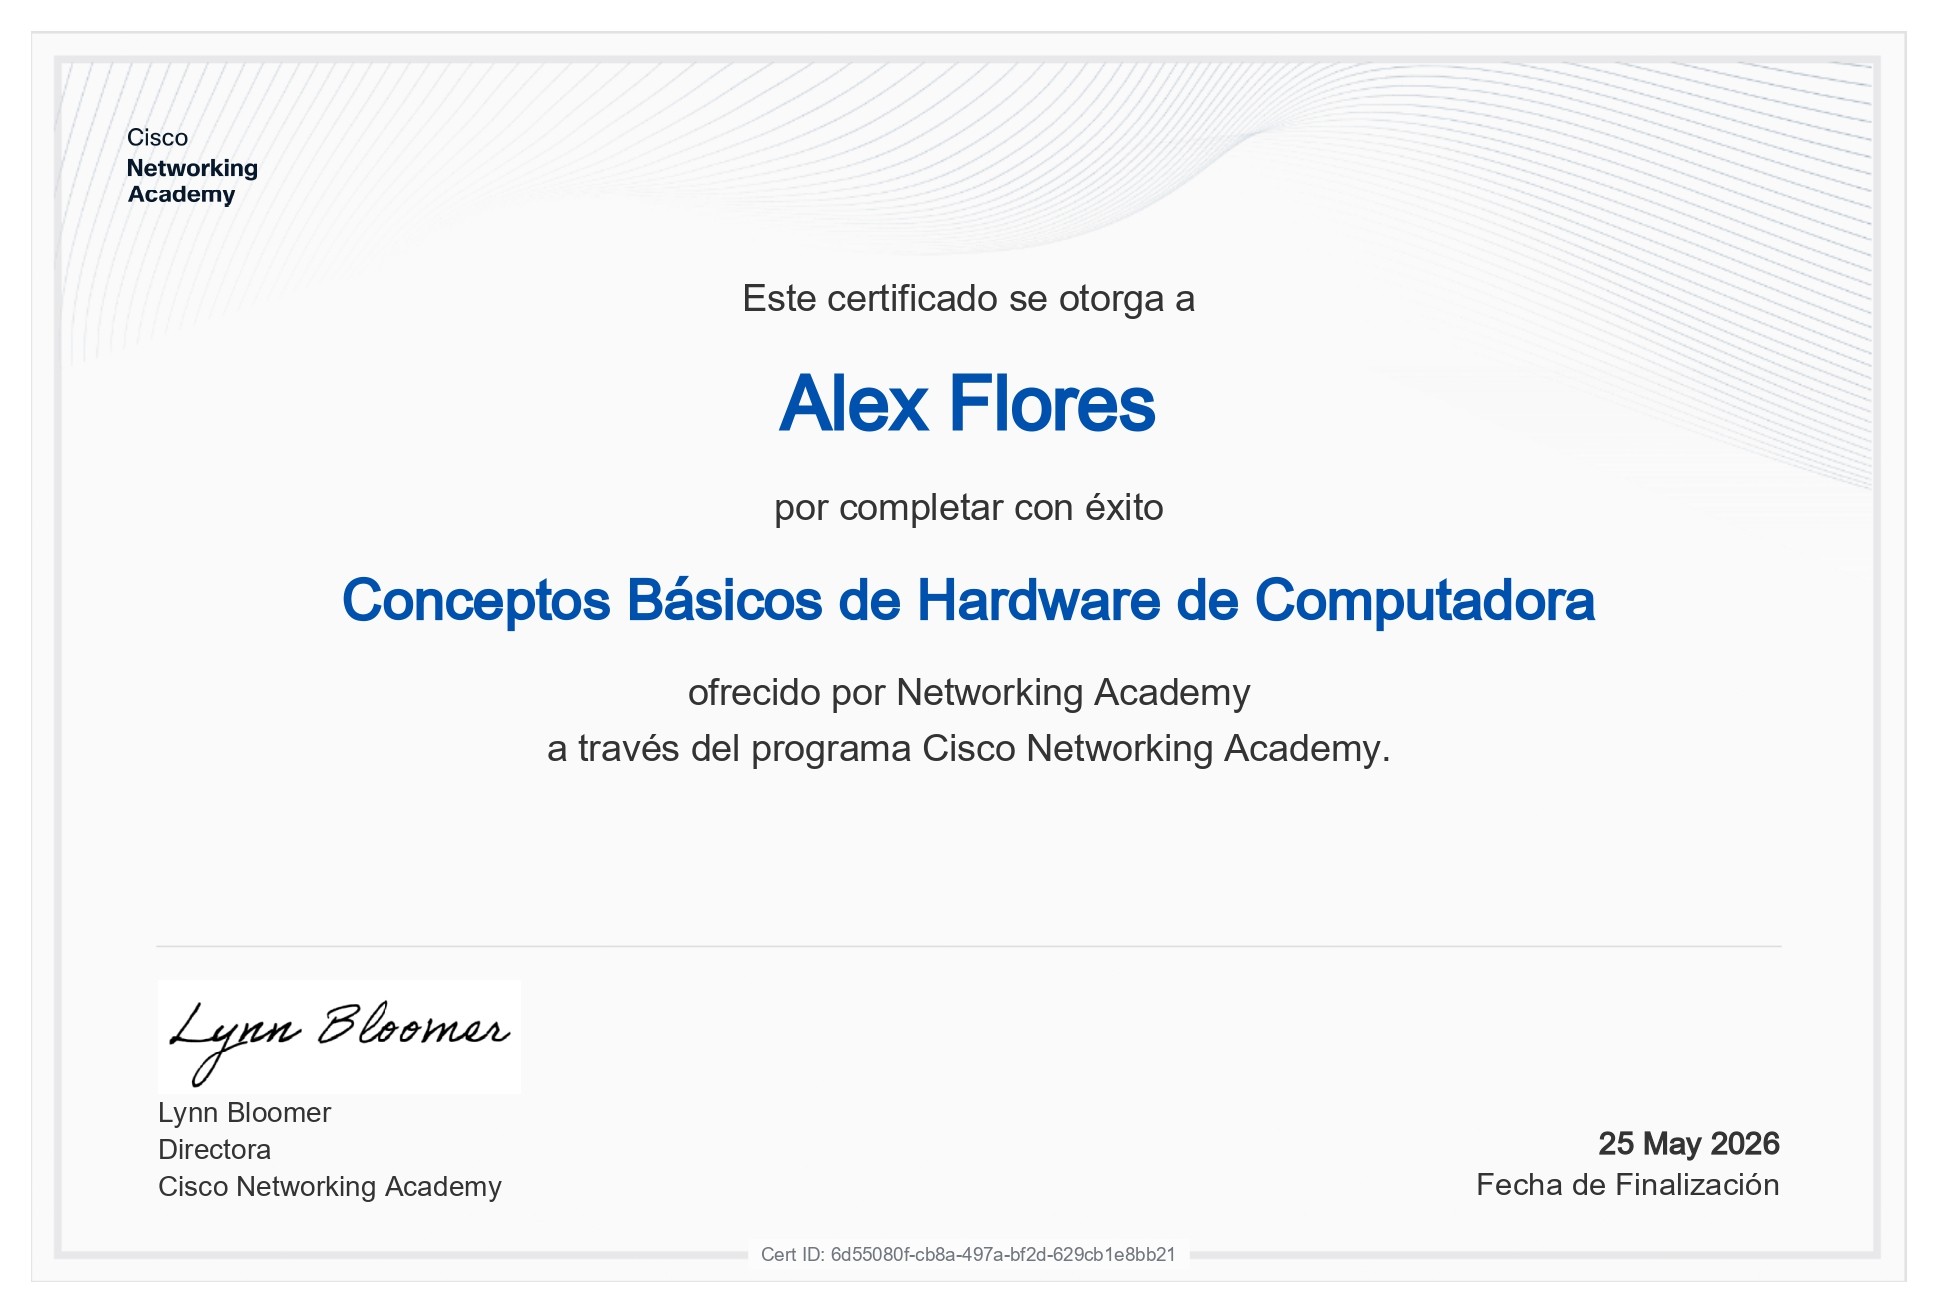
\includegraphics[width=.9\linewidth]{./images/Certificado_Alex.jpg}
\caption{\label{fig:org3d395b7}Certificado Alex Flores}
\end{figure}
\end{itemize}

\subsection{Integrante 3}
\label{sec:orgcf0adf1}
\begin{itemize}
\item \textbf{Nombre completo:} Micaela Dannae Sagñay Iza
\item \textbf{Correo:} micaela.sagnay@epn.edu.ec
\item \textbf{Certificado adjunto:}
\end{itemize}
\begin{center}
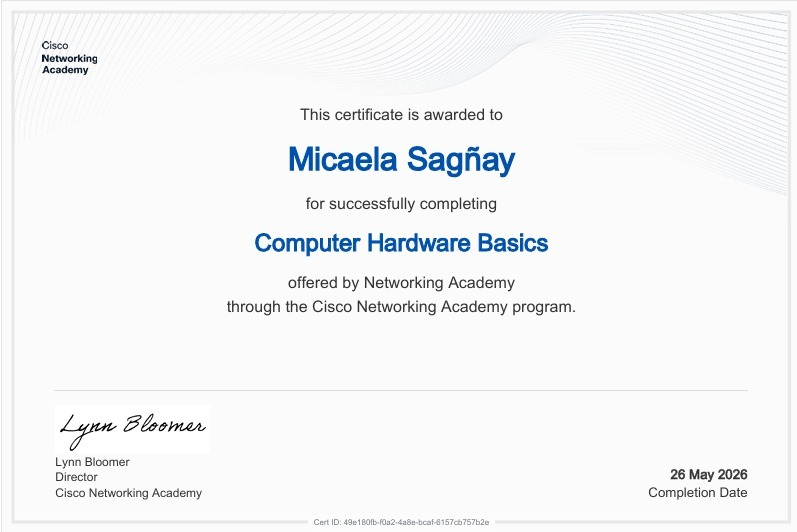
\includegraphics[width=.9\linewidth]{./images/certificado-micaela.jpg}
\label{org825cfbc}
\end{center}

\subsection{Integrante 4}
\label{sec:orgb4dd3ca}
\begin{itemize}
\item \textbf{Nombre completo:} Jami Tonato Mateo Israel
\item \textbf{Correo:} mateo.jami@epn.edu.ec
\item \textbf{Certificado adjunto:}     
\begin{figure}[htbp]
\centering
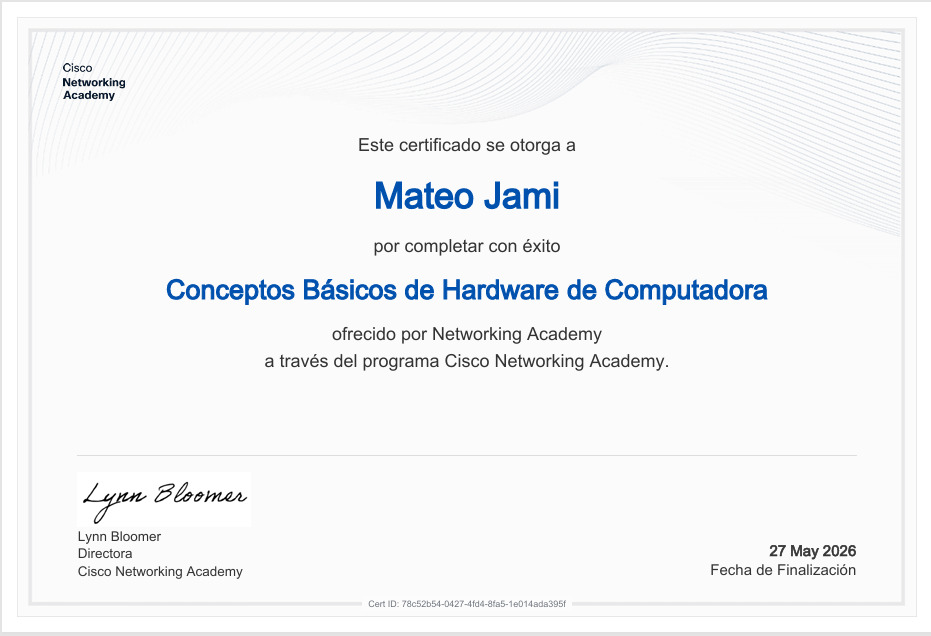
\includegraphics[width=.9\linewidth]{./images/Certificado_Mateo.jpg}
\caption{\label{fig:orgc3a1c81}Certificado Jami Mateo}
\end{figure}
\end{itemize}

\section{Parte B. Cuestionario argumentado grupal}
\label{sec:org460e958}

Para cada pregunta:

\begin{itemize}
\item Indique la alternativa escogida (letra).
\item Escriba una justificación técnica breve (3 a 6 líneas). Fundamente
su respuesta. Su insumo principal es el curso de Conceptos Básicos
de Hardware. Si usa otro material debe referenciar.
\item Discuta con el grupo de trabajo las opciones y la respuesta ¿Existió
consenso? ¿Cuáles fueron las principales discrepancias?
\end{itemize}

\textbf{Criterio:} correcto/incorrecto + calidad del argumento técnico.

\subsection{Pregunta 1}
\label{sec:org558936f}
Al instalar una CPU en un socket LGA, ¿por qué es crítico alinear el
pin 1 de la CPU con el pin 1 del socket?

a. Para que el sistema arranque con mayor rapidez 

b. Para evitar daños en la CPU y el socket al insertar incorrectamente

c. Porque el pin 1 es el único que conduce electricidad 

d. Para que el disipador quede centrado automáticamente

\begin{itemize}
\item \emph{Alternativa escogida:} Literal B
\item \emph{Justificación técnica:} En los sockets los pines están en el socket, no en la
CPU, alinear correctamente el pin 1 nos garantiza que el procesador se asiente
sin forzar, evitando doblar o romper pines del socket.
\item \emph{Debate del grupo:} Algunos consideraron inicialmente la opción A o D pero las
pudimos descartar esas opciones porque la velocidad de arranque y la alineacion
del disipador dependen de factores distintos, y la opción C es falsa ya que todos
los pines conducen señales y energía.
\end{itemize}
\subsection{Pregunta 2}
\label{sec:org53272e2}
Al montar la placa madre en el gabinete, ¿cuál es la función de los separadores (standoffs)?

a. Sostener el peso de las tarjetas de expansión

b. Evitar cortocircuitos entre la placa madre y el metal del gabinete

c. Mejorar la ventilación de la placa madre

d. Facilitar la alineación del panel de E/S trasero

\begin{itemize}
\item \emph{Alternativa escogida:} B
\item \emph{Justificación técnica:} Los separadores elevan la placa madre y crean un espacio
entre sus pistas de cobre y soldaduras y la bandeja metalica del gabinete, esto previene
contactos electricos no deseados que podrían provocar cortocircuitos o daños a la placa madre.
\item \emph{Debate del grupo:} Hubo una discusión sobre la opción D ya que al instalar los separadores
en los agujeros correctos si ayuda a que los puertos traseros coincidan con la chapa E/S, pero
su razón de ser fundamental es aislar electricamente la placa del chasis.
\end{itemize}

\subsection{Pregunta 3}
\label{sec:orgc10e2d4}
Según el manual de ensamblaje de Cisco, ¿cuándo NO es necesario aplicar pasta térmica al instalar el disipador sobre la CPU?

a. Cuando la CPU es de alto rendimiento

b. Cuando el disipador ya incluye pasta térmica preaplicada

c. Cuando la CPU tiene más de un año de uso

d. Cuando el gabinete tiene buena ventilación

\begin{itemize}
\item \emph{Alternativa escogida:} B
\item \emph{Justificación técnica:} La pasta termica es necesaria para llenar las microimperfecciones entre la superficie de la CPU
y la base del disipador, mejorando la transferencia de calor, muchos disipadores comerciales incluyen una capa
preaplicada, aplicar pasta adicional sobre una ya existente puede crear una capa demasiado gruesa
reduciendo la eficiencia térmica o incluso causando derrames sobre el socket.
\item \emph{Debate del grupo:} Hubo un descarte entre todas las opciones excepto la B, la opcion A, los CPUS de alto rendimiento
si requiere pasta, en la opción C la antiguedad del CPU no es relevante, si se reinstala un disipador usado
si debe limpiarse y aplicar pasta nueva pero eso no es no aplicar, en la opcion D, la ventilacion del gabinete
no reemplaza la necesidad de contacto térmico adecuado.
\end{itemize}

\subsection{Pregunta 4}
\label{sec:org67439e4}
¿Por qué se recomienda usar pulsera antiestática y alfombrilla antiestática al manipular componentes internos?

a. Para proteger al técnico de descargas de 220 V

b. Para evitar que la electricidad estática dañe los componentes

c. Para cumplir una norma estética del laboratorio

d. Para que los tornillos no se magneticen

\begin{itemize}
\item \emph{Alternativa escogida:} B
\item \emph{Justificación técnica:} La pulsera antiestática que está conectada
a tierra y la alfombrilla antiestática disipan de forma segura
cualquier diferencial de potencial, protegiendo los componentes
durante el manejo de los mismos, esto se enseña en el curso de Cisco
IT Essentials como una medida obligatoria antes e manipular hardware interno.
\item \emph{Debate del grupo:} En el grupo discutimos y estuvimos de acuerdo en
que la opción B era la correcta, se descartó la A porque la pulsera
antiestática no protege contra voltajes de red 220 V, para eso se
usan guantes dieléctricos y herramientas aisladas, se descartó la
opción C porque no es un tema estético, sino de seguridad del
hardware y se descartó la opción D porque los tornillos se
magnetizan por otros motivos, no por falta de antiestática.
\end{itemize}
\subsection{Pregunta 5}
\label{sec:org545fc05}
Si al iniciar la computadora por primera vez un LED del panel frontal no funciona, ¿qué indica el manual de Cisco?

a. Reemplazar el conector por uno de repuesto

b. Revisar el BIOS para habilitar el LED

c. Quitar el conector, invertirlo y volver a conectarlo

d. Desconectar y reconectar la fuente de poder

\begin{itemize}
\item \emph{Alternativa escogida:} C
\item \emph{Justificación técnica:} Los LED del panel frontal tienen polaridad,
si se conectan al revés no se encienden pero no se dañan los
componentes, el manual de Cisco y los estándares de ensamblaje
indican que ante un LED que no funciona en el primer encendido, lo
primero es verificar la orientación del conector e invertirlo si es
necesario, los interruptores funcionan en cualquier orientación,
pero los LED si requieren polaridad correcta.
\item \emph{Debate del grupo:} Se descartó la opción A porque no existen
conectores de repuesto para el panel frontal, también se descartó la
opción B porque los LED del panel frontal no se
habilitan/deshabilitan desde el BIOS, son del hardware y por último,
se descartó la opción D porque desconectar la fuente de poder no
soluciona un problema de polaridad invertida en el conector del LED.
\end{itemize}

\subsection{Pregunta 6}
\label{sec:orga6bf365}
¿Por qué una GPU puede requerir un conector de alimentación PCIe adicional de la fuente de poder?

a. Porque la ranura PCIe no transmite señal de video

b. Porque las GPUs de alto rendimiento consumen más potencia de la que la ranura puede suministrar

c. Porque el conector PCIe solo funciona con tarjetas de red

d. Por el estándar de codificación de color de los cables SATA

\begin{itemize}
\item \emph{Alternativa escogida:} B
\item \emph{Justificación técnica:} La ranura PCle x16 puede suministrar hasta
75 vatios, sin embargo, las tarjetas gráficas de alto rendimiento
pueden consumir 150W, 250W o más, para cubrir esta demanda adicional
se necesitan conectores de alimentación PCle e 6 u 8 pines
directamente desde la fuente de poder.
\item \emph{Debate del grupo:} Se descartó la opción A porque la ranura PCle sí
transmite señal de video solo que no a suficiente potencia, se
descartó la opción C porque el conector PCle de alimentación es para
gráficos no para tarjetas de red y se descartó la opción D porque el
código de color de cables SATA no tiene relación con conectores PCle
de GPU.
\end{itemize}

\section{Parte C. Mantenimiento de computadores}
\label{sec:orgf8a6083}

\subsection{3.1 Insumos para mantenimiento preventivo}
\label{sec:orgd098286}
Liste al menos seis insumos y describa para qué sirve cada
uno. Revise el siguiente \href{https://youtu.be/3ri1BMV7XTM?si=bjYoDUUKuMWwj4Qg}{vídeo}.

\begin{center}
\begin{tabular}{ll}
Insumo & Uso principal\\[0pt]
\hline
Aire comprimido & Eliminar polvo de componentes y ventiladores\\[0pt]
Alcohol isopropílico & Limpiar componentes electrónicos sin dañarlos\\[0pt]
Brocha antiestática & Retirar polvo de tarjetas y partes delicadas\\[0pt]
Pasta térmica & Mejorar la transferencia de calor del procesador\\[0pt]
Paño de microfibra & Limpiar pantallas y superficies\\[0pt]
Pulsera antiestática & Evitar descargas eléctricas en los componentes\\[0pt]
\end{tabular}
\end{center}

\subsection{3.2 Procedimiento de limpieza — Desktop}
\label{sec:org47992f8}
1.Apagar y desconectar el computador de la corriente.
2.Abrir el case con cuidado utilizando herramientas adecuadas.
3.Retirar el polvo interno usando aire comprimido y brocha antiestática.
4.Limpiar ventiladores, memoria RAM y demás componentes.
5.Cerrar el equipo y verificar su correcto funcionamiento.

\subsection{3.3 Procedimiento de limpieza — Laptop}
\label{sec:orgfb39115}
1.Apagar la laptop y desconectar el cargador.
2.Retirar la tapa inferior cuidadosamente.
3.Limpiar ventiladores y salidas de aire con aire comprimido.
4.Limpiar teclado, pantalla y superficie externa con paño de microfibra.
5.Ensamblar nuevamente la laptop y comprobar su funcionamiento.

\section{Parte D. Aprendizaje obtenido}
\label{sec:org29d21ea}

\subsection{Integrante 1 [Jhanavi Molina]}
\label{sec:org30c2c8c}
\begin{itemize}
\item \textbf{¿Qué conocimiento nuevo obtuvo del curso?} [Aprendí a identificar los componentes principales de una computadora como el CPU, memoria RAM, placa madre, disco duro y fuente de poder, tambien aprendí como se los ensambla correctamente.]
\item \textbf{¿Qué concepto corrigió o clarificó?} [Entendí que la pasta térmica no es opcional, si no necesaria para que la CPU no se sobrecaliente, antes no sabía o no tenía claro el concepto de para que servia.]
\end{itemize}
\subsection{Integrante 2 [Alex Flores]}
\label{sec:org811ffc8}
\begin{itemize}
\item \textbf{¿Qué conocimiento nuevo obtuvo del curso?} [Aprendí lo basico sobre mantenimiento tanto de PCs de escritorio como de laptops, tambien aprendi mas a fondo sobre los componentes, algunas buenas practicas de ensamblaje y limpieza de componentes]
\item \textbf{¿Qué concepto corrigió o clarificó?} [Me quedó mas claro como funcionan los componentes como RAM o procesador a nivel hardware, algunas practicas malas que tenia como claras en mi cabeza se aclararon y tambien corregi la manera de manipular los componentes]
\end{itemize}

\subsection{Integrante 3 [Micaela Sagñay]}
\label{sec:org2c8d91c}
\begin{itemize}
\item \textbf{¿Qué conocimiento nuevo obtuvo del curso?} [Obtuve conocimientos fundamentales sobre el mantenimiento preventivo y correctivo tanto en computadoras de escritorio como en laptops, además de profundizar en la arquitectura interna de los componentes y las normativas de seguridad para el ensamblaje.]
\item \textbf{¿Qué concepto corrigió o clarificó?} [Clarifique el funcionamiento a nivel de hardware de los componentes críticos como la memoria RAM y el procesador, además de corregir prácticas incorrectas de manipulación de componentes, adoptando técnicas adecuadas de limpieza y manejo de hardware.]
\end{itemize}

\subsection{Integrante 4 [Mateo Jami]}
\label{sec:orgc51f8db}
\begin{itemize}
\item \textbf{¿Qué conocimiento nuevo obtuvo del curso?} En este curso, logré
aprender algo más que solo los principios básicos del hardware de
un ordenador ya que fue bastante interesante saber el tipo de
herramientas necesarias para los mantenimientos, junto con los
cuidados que hay que tener para evitar daños permanentes en los
componentes del ordenador y esperaría a futuro poder incrementar
las bases que ahora tengo del hardware del ordenador.
\item \textbf{¿Qué concepto corrigió o clarificó?} No me quedaba del todo
claro el porque se utilizaban las conexiones a tierra en los
protectores antiestáticos y luego de aprobar el curso, usar su
material e investigar otros factores adicionales, logré
clarificar por completo la importancia de estas medidas de
protección al momento de manipular los componentes físicos del ordenador.
\end{itemize}


\section{Rúbrica de evaluación}
\label{sec:orgcbefe8a}

\begin{center}
\begin{tabular}{lr}
Criterio & Puntaje máximo\\[0pt]
\hline
Certificados individuales completos & 20\\[0pt]
Cuestionario: respuesta correcta (x8) & 30\\[0pt]
Cuestionario: argumento técnico (x8) & 30\\[0pt]
Mantenimiento (tabla + procedimientos) & 20\\[0pt]
TOTAL & 100\\[0pt]
\end{tabular}
\end{center}

\section{¿Cómo referenciar en Emacs?}
\label{sec:orgda9edb2}
Para insertar una referencia a un recurso bibliográfico
\begin{enumerate}
\item Puede actualizar el archivo \texttt{../bibliography/bibliography.bib}
\item Escribir en formato \textbf{\textbf{BibTeX}} el recurso bibliográfico
\item Verifique la siguiente configuración al encabezado:
\begin{verbatim}
   #+cite_export: biblatex
   #+LATEX_HEADER: \usepackage[backend=biber, style=ieee]{biblatex}
   #+BIBLIOGRAPHY: ../bibliography/bibliography.bib
\end{verbatim}
\item Usar \texttt{M-x org-cite-insert} para insertar una cita. Aparecerá una
lista. Use los cursores para seleccionar la cita. Ejecute \texttt{C-RET}: \emph{De acuerdo con
\autocite{ledin2022modern}, la arquitectura \ldots{}..}
\item Revise que al final del documento exista \texttt{\#+print\_bibliography:}
\item \textbf{\textbf{Sugerencia:}} Para evitar repetir varias veces el proceso de
exportación, es recomendable cambiar el compilador de \LaTeX a
\texttt{latexmk}. Para esto:
\begin{itemize}
\item \texttt{sudo apt install latexmk}
\item Revise en el encabezado del \texttt{.org} que el compilador escogido sea
\texttt{\#+LATEX\_COMPILER: latexmk}. También puede modificar el archivo
\texttt{init.el} para indicar qué compilador se usa para exportar de
\texttt{.org} a \emph{\LaTeX{}}:
\begin{verbatim}
;; 4.7b Proceso de compilación con latexmk para Org-export
(with-eval-after-load 'ox-latex
  (setq org-latex-pdf-process
        '("latexmk -f -pdf -%latex -interaction=nonstopmode -output-directory=%o %f")))

;; 4.7c Org-cite: biblatex como procesador para exportación LaTeX
(with-eval-after-load 'oc
  (setq org-cite-export-processors
        '((latex biblatex)
          (t basic))))

\end{verbatim}
\end{itemize}
\end{enumerate}
\section{Verificación de Entregables [100\%]:}
\label{sec:orgb3ab7bf}
Ejecute \texttt{C-c C-c} sobre los ítems de tarea según se hayan cumplido o
no. Si un ítem no pudo realizarse apunte en la siguiente sección las
razones al respecto.
\begin{itemize}
\item[{$\boxtimes$}] Los enlaces a los certificados en el documento \texttt{.org} funcionan.
\item[{$\boxtimes$}] Resolución completa del Cuestionario2.
\item[{$\boxtimes$}] Revisión del vídeo sobre mantenimiento a computador ASUS.
\item[{$\boxtimes$}] Tutorial de Comandos Emacs realizado.
\item[{$\boxtimes$}] Lista de insumos para mantenimiento completa.
\item[{$\boxtimes$}] Procedimiento de mantenimiento para desktop completo.
\item[{$\boxtimes$}] Procedimiento de mantenimiento para laptop completo.
\item[{$\boxtimes$}] Revisión de ortografía con \texttt{ispell-buffer} en el buffer
\item[{$\boxtimes$}] Generación de Archivo PDF \texttt{M-x org-latex-export-to-pdf}
\item[{$\boxtimes$}] Subir al aula virutal archivo \texttt{.org} y \texttt{.pdf}
\end{itemize}

\printbibliography
\end{document}
